\documentclass[a4paper, 12pt, finnish]{article}
\usepackage{babel}
\usepackage[utf8]{inputenc}
\usepackage[T1]{fontenc}
\usepackage{amsmath}
\usepackage{geometry}
\geometry{a4paper}
\usepackage{graphicx}
\usepackage{float}
\usepackage{wrapfig}
\usepackage{caption}
\usepackage{eurosym}
\usepackage[section]{placeins}
\usepackage{url}
\usepackage[hidelinks]{hyperref}
\usepackage{hyperref}
\usepackage{subcaption}
\usepackage{lipsum}
\usepackage[table,xcdraw]{xcolor}  
\usepackage{hyperref}
\usepackage{tabularx}
\hypersetup{
    colorlinks=true,
    linkcolor=black,
    urlcolor=blue,
}
\renewcommand{\figurename}{Kaavio }
\addto\captionsfinnish{\renewcommand{\figurename}{Kaavio}}
\def\UrlBreaks{\do\/\do-} %% Line breakit urleissa
\begin{document}
\title{MX Linux 18 käyttöönotto, käyttö ja ohjeistus \\ \large Projektisuunnitelma}
\author{Iiro Aarnio\\ Tampereen seudun ammattiopisto}
\maketitle
\thispagestyle{empty}
\newpage
\thispagestyle{empty}
\newpage
\begin{table}[htpb]
\begin{tabular}{llll}
Versiohistoria &            &                         &             \\
\rowcolor[HTML]{FFCCC9}
Versio         & Päivämäärä & Muutosperuste           & Tekijä      \\
0.1              & 4.6.2019   & Suunnitelman aloitus, työvaihekaavio       & Iiro Aarnio \\
1.0 & 4.6.2019 & Valmis esitettäväksi johtoryhmälle & Iiro Aarnio \\
\end{tabular}
\end{table}

%\begin{table}[h:wtpb]
%\begin{tabular}{lll}
%Jakelu &            &                                  \\
%\rowcolor[HTML]{FFCCC9}
%Tekijä         & Tulostettu & Jakelu                 \\
%Iiro Aarnio              & Ei ole   & Leena Järvenkylä-Niemi \\
%\end{tabular}
%\end{table}
\newpage
%%%%%%%%%%%%%%%%%%%%%           Table of Contents
\thispagestyle{empty}
\tableofcontents
\newpage
%%%%%%%%%%%%%%%%%%%%%           Table of Contents
\pagenumbering{arabic}
\section{Tehtävä}
Projektin tehtävänä on opiskella MX Linux 18 -GNU/Linux-jakelun käyttö, ja tehdä siitä käyttäjäystävällinen ohjekirja. Ohjekirja sisältää jakelun käyttöönoton, käyttäjähallinnan ja ohjelmienhallinnan ohjeet, ja muutaman yleisimmän työohjelman esittelyn. Opas kasataan yhdeksi loogiseksi kokonaisuudeksi, joka etenee järkevässä järjestyksessä.

\section{Tulostavoitteet}
Tehtävä on valmis kun on laadittu MX Linux 18 -jakelun käyttöönotosta ja peruskäytöstä tarkka sekä laaja ohjekirja, ja kun päätöspalaveri on pidetty.
\\\\
Laatutavoite: projektin dokumentaatiossa pyritään noudattamaan selvää suomen kieltä.

\section{Rajaukset}
Projektiin eivät kuulu laitteiston käyttöönotto, oheislaitteiden käyttöönotto, laitteistoajureiden opastus, tietoturvaohjeistus eikä asennusmedian luonnin opastus.
\section{Työvaiheet}
Työvaiheita on kuvattu seuraavassa kaaviossa.
\begin{figure}[!htpb]
    \centering
    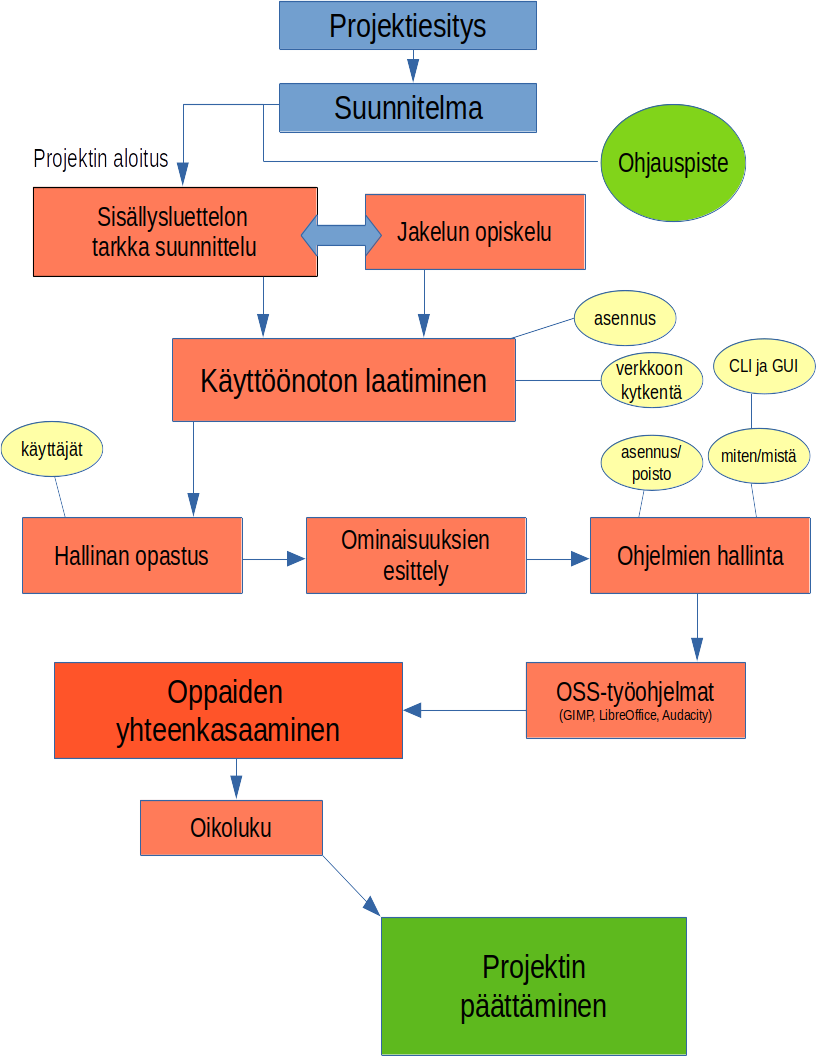
\includegraphics[width=\textwidth]{kaaviokuva}
    \caption{Työvaiheet}
    \label{}
\end{figure}

\section{Dokumentit ja tiedostojen säilöminen}

\subsection{Dokumentit}

Työstä luodaan ja tallennetaan sähköisessä muodossa seuraavat dokumentit:
\begin{itemize}
    \item jokaisen työntekijän tuntiseuranta 10 minuutin tarkkuudella
    \item edistymisraportit
    \item alustavat suunnitelmat kirjallisina
    \item MX Linux 18 ohjekirja
    \item loppuraportti
\end{itemize}

\subsection{Tallennukset}

Työt tallennetaan julkisesti nähtäväksi verkkoon. Tallennukseen ja säilytykseen käytetään Github-palvelua. \href{http://github.com/maysion/mxlinux18}{Linkki säilytyspaikkaan}. 

\section{Riskit ja keskeyttämiskriteerit}
\subsection{Henkilöstöön liittyvät riskit}
\begin{table}[!htpb]
\begin{tabularx}{1.1\textwidth}{|X|X|X|X|X|X|}
\hline
\rowcolor[HTML]{EFEFEF} 
\textbf{Riski} & \textbf{Vakavuus (1-5)} & \textbf{Toden-näköisyys (1-5)} & \textbf{Ensioire} & \textbf{Miten välttää} & \textbf{Miten selviytyä toteutuessa} \\ \hline
Henkilön sairastuminen & 5 & 3 & Kirjataan ylös sairastuminen ja tekemättä jääneet tehtävät &  & Jos aikataulu ei veny tarpeen mukaan, kartoitetaan turhimmat tehtävät ja poistetaan ne. \\ \hline
\end{tabularx}
\end{table}
\clearpage
\subsection{Laitteisiin liittyvät riskit}
\begin{table}[!htpb]
\begin{tabularx}{1.1\textwidth}{|X|X|X|X|X|X|}
\hline
\rowcolor[HTML]{EFEFEF} 
\textbf{Riski} & \textbf{Vakavuus (1-5)} & \textbf{Toden-näköisyys (1-5)} & \textbf{Ensioire} & \textbf{Miten välttää} & \textbf{Miten selviytyä toteutuessa} \\ \hline
Tiedostojen häviäminen & 5 & 1 & Tiedostojen puute & Tiedostot varmuuskopioidaan & Hävinneet tiedostot korvataan. \\ \hline
\end{tabularx}
\end{table}

\subsection{Hallintaan liittyvät riskit}
\begin{table}[!htpb]
\begin{tabularx}{1.1\textwidth}{|X|X|X|X|X|X|}
\hline
\rowcolor[HTML]{EFEFEF} 
\textbf{Riski} & \textbf{Vakavuus (1-5)} & \textbf{Toden-näköisyys (1-5)} & \textbf{Ensioire} & \textbf{Miten välttää} & \textbf{Miten selviytyä toteutuessa} \\ \hline
Työmäärän ylittyminen arvioista & 4 & 2 & Myöhästy-minen aikataulusta & Aikataulun seuraaminen & Tilanteen vaatiessa tulostavoitteita pienennetään. \\ \hline
\end{tabularx}
\end{table}

\section{Kustannukset}
Projektista ei odoteta tulevan rahallisia kustannuksia.

\section{Työmääräarvio ja resurssit}
Resurssihenkilöitä on projektitiimissä yksi. Arvioitu tuntityömäärä on noin 80 tuntia.



\end{document}
